\newpage
\section{Trigonometriske funktioner}
\begin{enumerate}
	\item Svarene er:
	\begin{align*}
	\frac{\pi}{2},&& \frac{\pi}{12},&&\frac{5\pi}{6},&& \frac{\pi}{4}.
	\end{align*}
	
	\item Svarene er:
	\begin{align*}
	60^\circ,&&315^\circ,&& 75^\circ.
	\end{align*}
	

	\begin{figure}
		\centering
		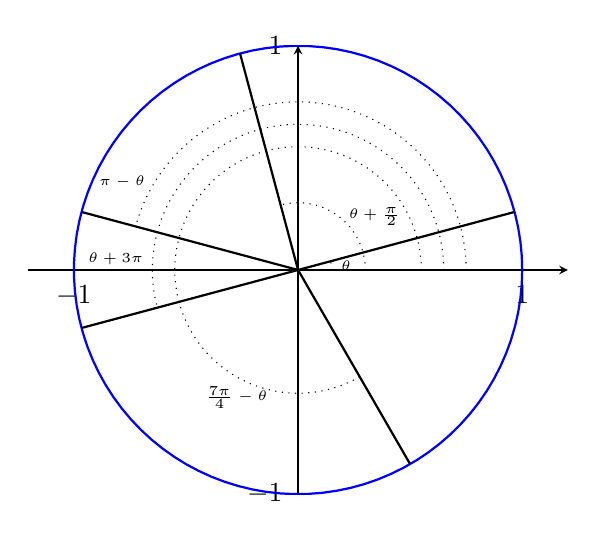
\begin{tikzpicture}
		\begin{axis}[xmin=-1,xmax=1,ymin=-1,ymax=1,axis x line=center,
		axis y line=center, axis equal,xtick={-1,1},ytick={-1,1}]
		\addplot[blue,domain=0:2*pi,thick, samples=100] ({cos(deg(x))},{sin(deg(x))});
		\addplot[domain=0:(sqrt(6)+sqrt(2))/4,thick] {(2-sqrt(3))*x};
		\addplot[domain=0:pi/12,samples=100,dotted] ({0.15*cos(deg(x))},{0.15*sin(deg(x))}) node[pos=0.5,right] {\tiny$\theta$};
		
		\addplot[domain=-(sqrt(6)-sqrt(2))/4:0,thick] {-1/(2-sqrt(3))*x};
		\addplot[domain=0:7*pi/12,samples=100,dotted] ({0.3*cos(deg(x))},{0.3*sin(deg(x))}) node[pos=0.5,right] {\tiny$\theta+\frac{\pi}{2}$};
		
		\addplot[domain=-(sqrt(6)+sqrt(2))/4:0,thick] {-(2-sqrt(3))*x};
		\addplot[domain=0:11*pi/12,samples=100,dotted] ({0.75*cos(deg(x))},{0.75*sin(deg(x))}) node[pos=0.9,left] {\tiny$\pi-\theta$};
		
		\addplot[domain=-(sqrt(6)+sqrt(2))/4:0,thick] {(2-sqrt(3))*x};
		\addplot[domain=0:13*pi/12,samples=100,dotted] ({0.65*cos(deg(x))},{0.65*sin(deg(x))}) node[pos=0.9,left] {\tiny$\theta+3\pi$};
		
		\addplot[domain=0:1/2,thick] {-sqrt(3)*x};
		\addplot[domain=0:5*pi/3,samples=100,dotted] ({0.55*cos(deg(x))},{0.55*sin(deg(x))}) node[pos=0.8,below] {\tiny$\frac{7\pi}{4}-\theta$};
		\end{axis}
		\end{tikzpicture}
		\caption{Opgave~\ref{it:trig1}}
		\label{fig:trig1ans}
	\end{figure}
	
	\item Svarene er:
	\begin{enumerate}
		\item Bestem $\sin(0)=0$ og $\cos(0)=1$.
		\item Bestem $\sin(\frac{\pi}{2})=1$ og $ \cos(\frac{\pi}{2})=0 $.
		\item Bestem $\sin(\pi)=0$ og $\cos(\pi)=-1$.
		\item Bestem $\sin(\frac{3\pi}{2})=-1 $ og $\cos(\frac{3\pi}{2})=0$.
		\item Bestem $\sin(2\pi)=0$ og $ \cos(2\pi) =1$.
	\end{enumerate}

	  
\item Svarene er:
\begin{align*}
0,&& \frac{3+2\sqrt{3}}{6},&& \frac{2\sqrt{3}}{3}.
\end{align*}
	
	\item Vi får at
	\begin{align*}
	\cos(-\theta)=\cos(0-\theta)=\cos(0)\cos(\theta)+\sin(0)\sin(\theta)=\cos(\theta),
	\end{align*}
	og 
	\begin{align*}
	\sin(-\theta)=\sin(0-\theta)=\sin(0)\cos(\theta)- \cos(0)\sin(\theta)=-\sin(\theta).
	\end{align*}
	
	\item Vi har at
	\begin{align*}
	\cos(\theta-\frac{\pi}{2})=\cos(\theta)\cos(\frac{\pi}{2})+\sin(\theta)\sin(\frac{\pi}{2})=\sin(\theta).
	\end{align*}
	  
	  	\item \label{it:trig1ans} Se Figur~\ref{fig:trig1ans} for en skitse af vinklerne
	  \begin{align*}
	  \theta+ \frac{\pi}{2},&& \pi-\theta,&& \theta +3\pi,&& \frac{7\pi}{4}-\theta.
	  \end{align*}

	 
	 \item Svarene kan være:
	 \begin{align*}
	 x=\frac{\pi}{3},x=\frac{2\pi}{3},&& x=\frac{\pi}{4},x=\frac{3\pi}{4},&& x=-\frac{\pi}{6},x=\frac{7\pi}{6}.
	 \end{align*}

	\item Indtegner man vinklen $x$ i enhedscirklen dannes en retvinklet trekant med kateter $\cos x$, $\sin x$ og hypotenuse $1$. Dermed giver Pythagoras sætning at
	\begin{align*}
	\sin^2x+\cos^2x=1.
	\end{align*}

	\item Svarene er:
	\begin{align*}
	-\frac{\sqrt{2}}{2},&& \frac{1}{2},&&1,&& \frac{1}{2}.
	\end{align*}
	
	\item\label{it:trig2} Vi har at 
	\begin{align*}
	\sin(2\theta)=\sin(\theta+\theta)=\sin(\theta)\cos(\theta)+\sin(\theta)=2\sin(\theta)\sin(\theta).
	\end{align*}

	\item Hvis vi bruger hintet får vi at ligningen reducerer til
	\begin{align*}
	(2\sin(2x))^2=3,\quad\Leftrightarrow\quad \sin(2x)=\pm \frac{\sqrt{3}}{2}.
	\end{align*}
	Hvis vi finder de vinkler $x\in [0,\pi]$, hvor $\sin(2x)=\pm\frac{\sqrt{3}}{2}$ får vi	$x=\frac{\pi}{6}$, $x=\frac{\pi}{3}$, $x=\frac{2\pi}{3}$, $x=\frac{5\pi}{6}$.
	
	
	\item Svarene er:
	\begin{align*}
	\frac{\sqrt{2}}{2},&& \sqrt{3},&& \frac{\sqrt{3}}{2},&& 0.
	\end{align*}
	
	\item Vi har at 
	\begin{align*}
	\frac{\sin(x+\pi)}{\cos(x+\pi)}=\frac{\sin(x)\cos(\pi)+\sin(\pi)\cos(x)}{\cos(x)\cos(\pi)-\sin(x)\sin(\pi)}=\frac{\sin(x)\cos(\pi)}{\cos(x)\cos(\pi)}=\frac{\sin x}{\cos x}.
	\end{align*}
	
	\item Bruger vi hintet reducerer ligningen til
	\begin{align*}
	\sin^2 x+ 3\cos^2 x=2\quad \Leftrightarrow\quad 1+2\cos^2 x=2\quad \Leftrightarrow\quad \cos x =\pm \frac{\sqrt{2}}{2}.
	\end{align*}
	Dermed er den eneste løsning i intervallet $[0,\frac{\pi}{2}]$ givet ved $x=\frac{\pi}{4}$.
	
	\item \label{it:trig3} Svarene kan være er:
	
	\begin{enumerate}
		\item Trekanten i Figur~\ref{fig:trig3} har en vinkel på $60$ grader og to af siderne har længde 1. Dermed må det være en ligesidet trekant hvor alle sidelængderne nødvendigvis er 1. Dette medfører at $\sin(\frac{\pi}{6})$, som er halvdelen af den lodrette stiplede linje, må være $\frac{1}{2}$.
		
		\item Idiotformlen giver, at $\sin^2 \frac{\pi}{6}+\cos^2\frac{\pi}{6}=1$ og ved at løse ligningen for $\cos(\frac{\pi}{6})$ får vi at $ \cos(\frac{\pi}{6})=\sqrt{1-\frac{1}{4}}=\frac{\sqrt{3}}{2} $.
		
		\item Ved at bruge formlen fra Opgave~\ref{it:trig2}
		\begin{align*}
		 \sin(\frac{\pi}{3})=\sin(2\frac{\pi}{6}) =2\sin(\frac{\pi}{6})\cos(\frac{\pi}{6})=2\frac{1}{2}\frac{\sqrt{3}}{2}=\frac{\sqrt{3}}{2}.
		\end{align*}
		
		\item Vi har at
		\begin{align*}
		\sin^2 \frac{\pi}{3}+ \cos^2\frac{\pi}{3}=1\quad \Leftrightarrow\quad \cos^2\frac{\pi}{3}=1-\frac{3}{4}\quad \Leftrightarrow\quad \cos\frac{\pi}{3}=\sqrt{\frac{1}{4}}=\frac{1}{2}.
		\end{align*}
		
	\end{enumerate}
		
	% \begin{figure}
	% 	\centering
	% 	\begin{tikzpicture}
	% 	\begin{axis}[xmin=-1,xmax=1,ymin=-1,ymax=1,axis x line=center,
	% 	axis y line=center, axis equal]
	% 	\addplot[blue,domain=0:2*pi,thick, samples=100] ({cos(deg(x))},{sin(deg(x))});
	% 	\addplot[domain=0:sqrt(3)/2,thick] {1/sqrt(3)*x};
	% 	\addplot[domain=0:pi/6,thick,samples=100] ({0.2*cos(deg(x))},{0.2*sin(deg(x))}) node[label={[label distance=2pt]0.5:\small$\frac{\pi}{6}$},pos=1] {};
	% 	\addplot[domain=0:sqrt(3)/2,thick,gray,dotted] {-1/sqrt(3)*x};
	% 	\addplot[domain=-pi/6:0,thick,samples=100,gray,dotted] ({0.2*cos(deg(x))},{0.2*sin(deg(x))}) node[label={[label distance=2pt]0.5:\small$\frac{\pi}{6}$},pos=0] {};
	% 	\addplot[dotted,gray,thick] coordinates {(sqrt(3)/2, -1/2) (sqrt(3)/2, 1/2)};
	% 	\end{axis}
	% 	\end{tikzpicture}
	% 	\caption{Opgave~\ref{it:trig3}}
	% 	\label{fig:trig3}
	% \end{figure}

		\item \label{it:trig4} Svarene kan være:
		\begin{enumerate}
			\item Da trekanten i Figur~\ref{fig:trig4} er retvinklet og begge kateter har længde $1$ kan vi anvende Pythagoras og få at hypotenusen har længde $\sqrt{1+1}=\sqrt{2}$. Da $\sin \frac{\pi}{4}$ er halvdelen af hypotenusen fås at $\sin\frac{\pi}{4}=\frac{\sqrt{2}}{2}$. 
			\item Vi har at
			\begin{align*}
			\cos \frac{\pi}{4}=\sqrt{1-\frac{1}{2}}=\frac{\sqrt{2}}{2}.
			\end{align*}
		\end{enumerate}
	
	% \begin{figure}
	% 	\centering
	% 	\begin{tikzpicture}
	% 	\begin{axis}[xmin=-1,xmax=1,ymin=-1,ymax=1,axis x line=center,
	% 	axis y line=center, axis equal]
	% 	\addplot[blue,domain=0:2*pi,thick, samples=100] ({cos(deg(x))},{sin(deg(x))});
	% 	\addplot[domain=0:sqrt(2)/2,thick] {1*x};
	% 	\addplot[domain=0:pi/4,thick,samples=100] ({0.2*cos(deg(x))},{0.2*sin(deg(x))}) node[label={[label distance=2pt]0.5:\small$\frac{\pi}{4}$},pos=1] {};
	% 	\addplot[domain=0:sqrt(2)/2,thick,gray,dotted] {-1*x};
	% 	\addplot[domain=-pi/4:0,thick,samples=100,gray,dotted] ({0.2*cos(deg(x))},{0.2*sin(deg(x))}) node[label={[label distance=2pt]0.5:\small$\frac{\pi}{4}$},pos=0] {};
	% 	\addplot[dotted,gray,thick] coordinates {({sqrt(2)/2}, -{sqrt(2)/2}) ({sqrt(2)/2}, {sqrt(2)/2})};
	% 	\end{axis}
	% 	\end{tikzpicture}
	% 	\caption{Opgave~\ref{it:trig4}}
	% 	\label{fig:trig4}
	% \end{figure}

	\item \label{it:trig5} Svarene kan være:
	\begin{enumerate}
%		\item Brug Figur~\ref{fig:trig5} at $\sin(\frac{\pi}{12})=\frac{\sqrt{2-\sqrt{3}}}{2}$. (Hint: Brug cosinusrelationen)
%		\item Brug idiotformlen til at bestemme $\cos(\frac{\pi}{12})$. 
		\item Vi bruger hintet og får
		\begin{align*}
		\sin\frac{\pi}{12}=\sin(\frac{\pi}{3})\cos(\frac{\pi}{4})-\sin(\frac{\pi}{4})\cos(\frac{\pi}{3})=\frac{\sqrt{3}}{2}\frac{\sqrt{2}}{2}-\frac{\sqrt{2}}{2}\frac{1}{2}=\frac{1}{4}(\sqrt{6}- \sqrt{2}).
		\end{align*}
		Gør vi det samme for cosinus får vi at
		\begin{align*}
		\cos \frac{\pi}{12}=\cos(\frac{\pi}{3})\cos(\frac{\pi}{4})+\sin(\frac{\pi}{4})\sin(\frac{\pi}{3})=\frac{1}{2}\frac{\sqrt{2}}{2}+\frac{\sqrt{2}}{2}\frac{\sqrt{3}}{2}=\frac{1}{4}(\sqrt{6}+ \sqrt{2}).
		\end{align*}
		
		\item Ved at bruge præcis samme fremgangsmåde som før får vi at 
		\begin{align*}
		\sin \frac{5\pi}{12}=\frac{1}{4}(\sqrt{6}+ \sqrt{2}),
		\end{align*}
		og 
		\begin{align*}
		\cos \frac{5\pi}{12}=\frac{1}{4}(\sqrt{6}- \sqrt{2}).
		\end{align*}
	\end{enumerate}
	
	
%	\begin{figure}
%		\centering
%		\begin{tikzpicture}
%		\begin{axis}[xmin=-1,xmax=1,ymin=-1,ymax=1,axis x line=center,
%		axis y line=center, axis equal]
%		\addplot[blue,domain=0:2*pi,thick, samples=100] ({cos(deg(x))},{sin(deg(x))});
%		\addplot[domain=0:(sqrt(6)+sqrt(2))/4,thick] {(2-sqrt(3))*x};
%		\addplot[domain=0:pi/12,thick,samples=100] ({0.2*cos(deg(x))},{0.2*sin(deg(x))}) node[label={[label distance=2pt]0.5:\tiny$\frac{\pi}{12}$},pos=1] {};
%
%		\addplot[domain=0:(sqrt(6)+sqrt(2))/4,thick,gray,dotted] {-(2-sqrt(3))*x};
%		\addplot[domain=-pi/12:0,thick,samples=100,gray,dotted] ({0.2*cos(deg(x))},{0.2*sin(deg(x))}) node[label={[label distance=2pt]0.5:\tiny$\frac{\pi}{12}$},pos=0] {};
%		\addplot[dotted,gray,thick] coordinates {({(sqrt(6)+sqrt(2))/4}, -{(sqrt(6)-sqrt(2))/4}) ({(sqrt(6)+sqrt(2))/4}, {(sqrt(6)-sqrt(2))/4})};
%		\end{axis}
%		\end{tikzpicture}
%		\caption{Opgave~\ref{it:trig5}}
%		\label{fig:trig5}
%	\end{figure}
%	

	
\end{enumerate}